\begin{center}
\Huge
	Ekstrema og monotoni
\end{center}
\section*{Ekstrema}
\stepcounter{section}

Et \textit{ekstremum} for en funktion er løst beskrevet det lokalt højeste eller laveste punkt på grafen for en funktion. Vi definerer to klasser af ekstrema mere præcist.
\begin{defn}[Ekstremum]
	Lad $f:A \to \mathbb{R}$ være givet. Hvis der for et $x_0 \in A$ gælder, at der findes et interval 
	$[x_0 - k,x_0 + k] \subseteq A$ så  
	\begin{align*}
		f(x_0) \geq f(x)
	\end{align*}
	for alle $x \in [x_0 - k, x_0 + k]$, så siges $x_0$ at være et \textit{lokalt maksimumssted} for $f$.
	Punktet $(x_0,f(x_0))$ kaldes for et \textit{lokalt maksimum}. Hvis det gælder, at 
	\begin{align*}
		f(x_0) \geq f(x)
	\end{align*}	
	for alle $x \in A$, så siges $x_0$ at være et \textit{globalt maksimumssted} for $f$.
	Punktet $(x_0,f(x_0))$ kaldes for et \textit{lokalt maksimum}. Gælder det modsat for et $x_0\in A$, at der
	findes et interval $[x_0 - k, x_0 + k]$ så 
	\begin{align*}
		f(x_0) \leq f(x)
	\end{align*}
	for alle $x \in [x_0 - k, x_0 + k]$, så siges $x_0$ at være et \textit{lokalt minimumssted} for $f$. 
	Punktet $(x_0,f(x_0))$ kaldes for et \textit{lokalt minimum.}
	Hvis det gælder, at 
	\begin{align*}
		f(x_0) \leq f(x)
	\end{align*}
	for alle $x \in A$, så siges $x_0$ af være et \textit{globalt minimumssted}. 
	Punktet $(x_0,f(x_0))$ kaldes for et \textit{globalt minimum}.
\end{defn}
På Figur \ref{fig:lokmax} kan vi se et interval omkring et lokalt maksimum og på Figur \ref{fig:ekstrema} kan vi se en række forskellige typer af ekstrema for en funktion.
\begin{figure}[H]
	\centering
	\begin{minipage}{0.48\textwidth}
	\centering
	\resizebox{0.95\textwidth}{!}{
	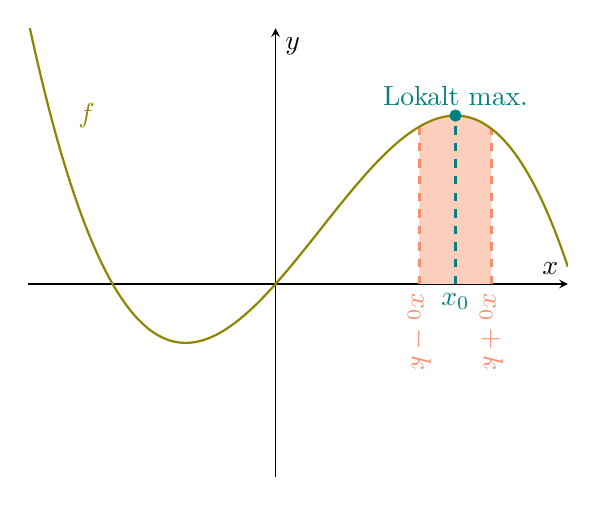
\begin{tikzpicture}
	\begin{axis}[
	axis lines = center, 
	xmin = -5.5, xmax = 6.5,
	ymin = -30.5, ymax = 40.5,
	xlabel = $x$, ylabel = $y$, 
	ticks = none,
	]
		\fill[color = Melon!40, variable = \x, domain = 3.2:4.8] (axis cs: 3.2,0) -- 
		plot (axis cs: \x, -1/3*\x^3 + \x^2 + 8*\x) -- (axis cs: 4.8,0) -- cycle;
		\draw[color = teal, thick, dashed] (axis cs: 4,0) -- (axis cs: 4,80/3);
		\draw[color = Melon, thick, dashed] (axis cs: 3.2,0) -- (axis cs: 3.2,24.9173);
		\draw[color = Melon, thick, dashed] (axis cs: 4.8,0) -- (axis cs: 4.8,24.576);
		\addplot[color = olive, thick, samples = 300, domain = -6.5:6.5] {-1/3*x^3 + x^2 + 8*x};
		\filldraw[color = teal] (axis cs:4,80/3) circle (2pt);
		\node[color = teal, anchor = north] at (axis cs: 4,0) {$x_0$};
		\node[color = Melon, anchor = west, rotate = -90] at (axis cs: 3.2,0) {$x_0 - k$};
		\node[color = Melon, anchor = west, rotate = -90] at (axis cs: 4.8,0) {$x_0 + k$};
		\node[color = teal, anchor = south] at (axis cs: 4,80/3) {Lokalt max.};
		\node[color = olive] at (axis cs: -4.2,80/3) {$f$};
	\end{axis}
	\end{tikzpicture}
	}
	\caption{Lokalt maksimum og interval omkring maksimum.}
	\label{fig:lokmax}
	\end{minipage}
	\begin{minipage}{0.48\textwidth}
	\centering
	\resizebox{0.95\textwidth}{!}{
	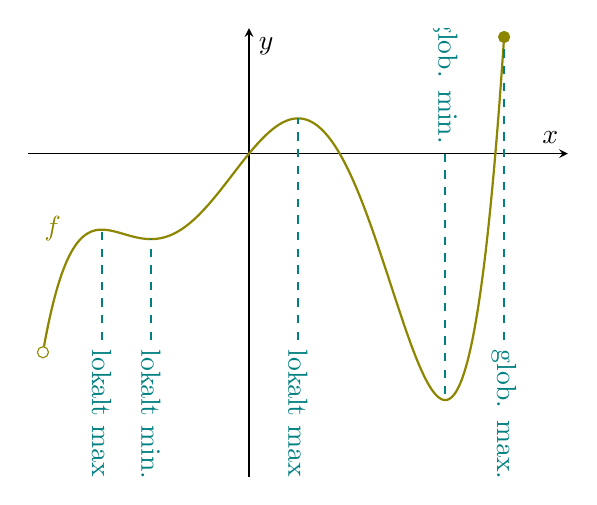
\begin{tikzpicture}
	\begin{axis}[
	axis lines = center, 
	xmin = -4.5, xmax = 6.5,
	ymin = -130, ymax = 50.5,
	xlabel = $x$, ylabel = $y$, 
	ticks = none,
	]
		\addplot[color = olive, thick, domain = -4.2:5.2, samples = 400] {24*x - 5*x^2 - 5*x^3 + 1/5*x^5};
		\node[color = teal, anchor = west, rotate = -90] at (axis cs: -3,-75) {lokalt max.};
		\draw[color = teal, dashed, thick] (axis cs: -3,-75) -- (axis cs:-3,-154/5); 
		\node[color = teal, anchor = west, rotate = -90] at (axis cs: -2,-75) {lokalt min.};
		\draw[color = teal, dashed, thick] (axis cs: -2,-75) -- (axis cs:-2,-172/5); 
		\node[color = teal, anchor = west, rotate = -90] at (axis cs: 1,-75) {lokalt max.};
		\draw[color = teal, dashed, thick] (axis cs: 1,-75) -- (axis cs:1,71/5); 
		\node[color = teal, anchor = east, rotate = -90] at (axis cs: 4,0) {glob. min.};
		\draw[color = teal, dashed, thick] (axis cs: 4,0) -- (axis cs: 4,-496/5); 
		\node[color = teal, anchor = west, rotate = -90] at (axis cs: 5.2,-75) {glob. max.};
		\draw[color = teal, dashed, thick](axis cs: 5.2,-75) --  (axis cs: 5.2,46.9681); 
		\filldraw[color = white]  (axis cs: -4.2, -79.9425) circle (2pt);
		\draw[color = olive]  (axis cs: -4.2, -79.9425) circle (2pt);
		\filldraw[color = olive]  (axis cs: 5.2, 46.9681) circle (2pt);
		\node[color = olive] at (axis cs: -4,-30) {$f$};
	\end{axis}
	\end{tikzpicture}
	}
	\caption{Forskellige ekstrema for en funktion.}
	\label{fig:ekstrema}
	\end{minipage}
\end{figure}

\section*{Monotoni}
\stepcounter{section}

Det kan være meningsfuldt at beskrive funktioner på intervaller, hvor de enten kun vokser eller kun aftager fx. i forbindelse med inverse funktioner. Hvis en funktion kun er voksende eller aftagende på et interval, siges funktionen at være \textit{monoton} på intervallet. Vi definerer det mere præcist.
\begin{defn}[Monotoni]
	En funktion $f$ siges at være \textit{voksende} på et interval $[a,b]$, hvis det for
	 $x_1,x_2\in [a,b]$, hvor $x_2 > x_1$, gælder, at 
	\begin{align*}
		f(x_2) \geq f(x_1).
	\end{align*}
	Hvis uligheden er skarp $(>)$, siges funktionen at være \textit{strengt voksende.} Modsat siges $f$ at være 
	aftagende på intervallet $[a,b]$, hvis det for $x_1,x_2 \in [a,b]$, hvor $x_2 > x_1$, gælder, at
	\begin{align*}
		f(x_2) \leq f(x_1).
	\end{align*}
	Hvis uligheden er skarp $(<)$, siges funktionen at være \textit{strengt aftagende.}
\end{defn}
Vi kan se grafen for en voksende funktion på Figur \ref{fig:voksende} og en aftagende funktion på Figur \ref{fig:aftagende}.
\begin{figure}[H]
	\centering
	\begin{minipage}{0.48\textwidth}
		\centering
		\resizebox{0.95\textwidth}{!}{
		\begin{tikzpicture}
		\begin{axis}[
		axis lines = center,
		xmin = -6.5,xmax = 6.5,
		ymin = -6.5,ymax = 6.5,
		xlabel= $x$, ylabel = $y$,
		ticks = none,
		]
			\addplot[color = olive, thick, samples = 300, domain = -6.5:6.5] {x + cos(deg(x))};
			\draw[color = teal, thick, dashed] (axis cs: 5,0) --  (axis cs: 5,5.2836);
			\draw[color = teal, thick, dashed] (axis cs: 0,5.2836) --  (axis cs: 5,5.2836);
			\draw[color = teal, thick, dashed] (axis cs: 1,0) --  (axis cs: 1,1.5403);
			\draw[color = teal, thick, dashed] (axis cs: 0,1.5403) --  (axis cs: 1,1.5403);
			\node[color = teal, anchor = east] at (axis cs: 0,1.5403) {$f(x_1)$};
 			\node[color = teal, anchor = east] at (axis cs: 0,5.2836) {$f(x_2)$};
 			\node[color = teal, anchor = north] at (axis cs: 1,0) {$x_1$};
 			\node[color = teal, anchor = north] at (axis cs: 5,0) {$x_2$};
 			\node[color = olive] at (axis cs: -4,-4) {$f$};
		\end{axis}
		\end{tikzpicture}
		}
		\caption{Graf for voksende funktion.}
		\label{fig:voksende}
	\end{minipage}
	\begin{minipage}{0.48\textwidth}
		\centering
		\resizebox{0.98\textwidth}{!}{
		\begin{tikzpicture}
		\begin{axis}[
		axis lines = center,
		xmin = -6.5,xmax = 6.5,
		ymin = -6.5,ymax = 6.5,
		xlabel= $x$, ylabel = $y$,
		ticks = none,
		]
			\addplot[color = olive, thick, samples = 300, domain = -6.5:6.5] {-x -cos(deg(x))};
			\draw[color = teal, thick, dashed] (axis cs: 5,0) --  (axis cs: 5,-5.2836);
			\draw[color = teal, thick, dashed] (axis cs: 0,-5.2836) --  (axis cs: 5,-5.2836);
			\draw[color = teal, thick, dashed] (axis cs: 1,0) --  (axis cs: 1,-1.5403);
			\draw[color = teal, thick, dashed] (axis cs: 0,-1.5403) --  (axis cs: 1,-1.5403);
			\node[color = teal, anchor = east] at (axis cs: 0,-1.5403) {$f(x_1)$};
 			\node[color = teal, anchor = east] at (axis cs: 0,-5.2836) {$f(x_2)$};
 			\node[color = teal, anchor = south] at (axis cs: 1,0) {$x_1$};
 			\node[color = teal, anchor = south] at (axis cs: 5,0) {$x_2$};
 			\node[color = olive] at (axis cs: -4,4) {$f$};
		\end{axis}
		\end{tikzpicture}
		}
		\caption{Graf for aftagende funktion.}
		\label{fig:aftagende}
	\end{minipage}
\end{figure} 

Vi kan for en funktion opskrive \textit{monotoniforholdene}, der er de intervaller, hvor en funktion $f$ er enten voksende eller aftagende. Vi betragter et eksempel.

\begin{exa}
	Grafen for en funktion $f$ kan ses på Figur \ref{fig:monotoni}.
	\begin{figure}[H]
		\centering
		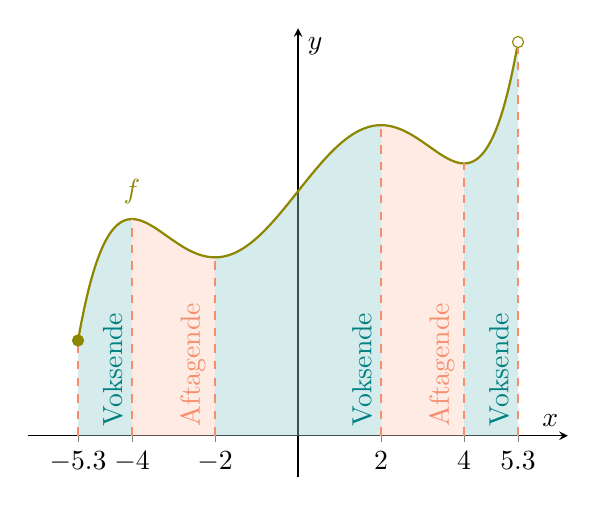
\begin{tikzpicture}
		\begin{axis}[
		axis lines = center,
		xmin = -6.5,xmax = 6.5,
		ymin = -50,ymax = 500,
		xlabel= $x$, ylabel = $y$,
		xtick = {-5.3,-4,-2,2,4,5.3},
		ytick = {0},
		]	
			%voksende
			\fill[color = teal!40, variable = \x, domain = -5.3:-4,opacity = 0.4] (axis cs:-5.3,0) --
			 plot (axis cs: \x, 64*\x - 20/3*\x^3 + 1/5*\x^5 + 300) -- (axis cs: -4,0) -- cycle;
			%aftagende
			\fill[color = Melon!40, variable = \x, domain = -4:-2,opacity = 0.4] (axis cs:-4,0) --
			 plot (axis cs: \x, 64*\x - 20/3*\x^3 + 1/5*\x^5 + 300) -- (axis cs: -2,0) -- cycle;
			%voksende
			\fill[color = teal!40, variable = \x, domain = -2:2, opacity = 0.4] (axis cs:-2,0) --
			 plot (axis cs: \x, 64*\x - 20/3*\x^3 + 1/5*\x^5 + 300) -- (axis cs: 2,0) -- cycle;
			%aftagende
			\fill[color = Melon!40, variable = \x, domain = 2:4,opacity = 0.4] (axis cs:2,0) --
			 plot (axis cs: \x, 64*\x - 20/3*\x^3 + 1/5*\x^5 + 300) -- (axis cs: 4,0) -- cycle;
			%voksende
			\fill[color = teal!40, variable = \x, domain = 4:5.3,opacity = 0.4] (axis cs:4,0) --
			 plot (axis cs: \x, 64*\x - 20/3*\x^3 + 1/5*\x^5 + 300) -- (axis cs: 5.3,0) -- cycle;
			\addplot[color = olive, thick, samples = 500, domain = -5.3:5.3] {64*x - (20*x^3)/3 + 1/5*x^5 + 300};
 			\node[color = olive] at (axis cs: -4,300) {$f$};
 			\draw[color = Melon, dashed, thick] (axis cs:-5.3,0) -- (axis cs:-5.3,116.922);
 			\draw[color = Melon, dashed, thick] (axis cs:-4,0) -- (axis cs:-4,265.867);
 			\draw[color = Melon, dashed, thick] (axis cs:-2,0) -- (axis cs:-2,218.933);
 			\draw[color = Melon, dashed, thick] (axis cs:2,0) -- (axis cs:2,381.067);
 			\draw[color = Melon, dashed, thick] (axis cs:4,0) -- (axis cs:4,334.133);
 			\draw[color = Melon, dashed, thick] (axis cs:5.3,0) -- (axis cs:5.3,483.078);
 			\filldraw[color = olive] (axis cs: -5.3,116.922) circle (2pt);
			\filldraw[color = white] (axis cs: 5.3,483.078) circle (2pt);
			\draw[color = olive] (axis cs: 5.3,483.078) circle (2pt);
			\node[color = teal, anchor = south west, rotate = 90] at (axis cs: -4,0) {Voksende};
			\node[color = Melon, anchor = south west, rotate = 90] at (axis cs: -2,0) {Aftagende};
			\node[color = teal, anchor = south west, rotate = 90] at (axis cs: 2,0) {Voksende};
			\node[color = Melon, anchor = south west, rotate = 90] at (axis cs: 4,0) {Aftagende};
			\node[color = teal, anchor = south west, rotate = 90] at (axis cs: 5.3,0) {Voksende};
		\end{axis}
		\end{tikzpicture}
		\caption{Graf for $f$ med monotone intervaller markeret.}
		\label{fig:monotoni}
	\end{figure}
	Vi kan nu opskrive monotoniforholdene for funktionen $f$.
	\begin{itemize}
		\item[$\cdot$] $f$ er voksende for $x \in [-5.3,-4]$.
		\item[$\cdot$] $f$ er aftagende for $x \in [-4,-2]$.
		\item[$\cdot$] $f$ er voksende for $x \in [-2,2]$.
		\item[$\cdot$] $f$ er aftagende for $x \in [2,4]$.
		\item[$\cdot$] $f$ er voksende for $x \in [4,5.3[$.
	\end{itemize}
	Vi kan også bruge foreningsmængden $\cup$ til at opskrive monotoniforholdene lidt mere kompakt.
	\begin{itemize}
		\item[$\cdot$] $f$ er voksende for $x \in [-5.3,-4] \cup [-2,2] \cup [4,5.3[$.
		\item[$\cdot$] $f$ er aftagende for $x \in [-4,-2] \cup [2,4]$.
	\end{itemize}
	I fald funktionen $f$ ikke er afgrænset til et begrænset interval, så ville funktionen blive ved med at 
	vokse. I så fald ville vi skrive $f$ er voksende for $x \in [4,+\infty[$.
\end{exa}

\newpage

\subsection*{Opgave 1}
Bestem ekstremumsstederne for følgende funktioner og afgør, om de er lokale eller globale minima.
\begin{center}
\resizebox{0.45\textwidth}{!}{
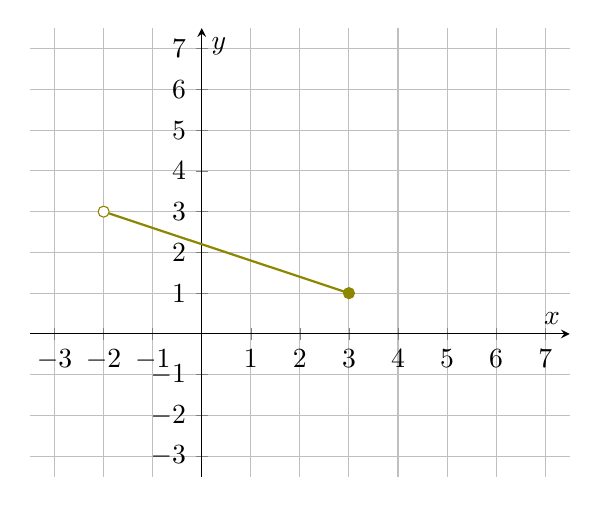
\begin{tikzpicture}
	\begin{axis}
	[axis lines = center, 
	xmin = -3.5, xmax = 7.5,
	ymin = -3.5, ymax = 7.5,
	grid = both,
	xtick = {-3,-2,...,6,7},
	ytick = {-3,-2,...,6,7},
	xlabel = $x$, ylabel = $y$
	]
		\addplot[color = olive, thick, domain = -2:3] {-2/5*x+2.2};	
		\filldraw[color = white](axis cs: -2,3) circle (2pt);
		\filldraw[color = olive](axis cs: 3,1) circle (2pt);
		\draw[color = olive](axis cs: -2,3) circle (2pt);
	\end{axis}
\end{tikzpicture}
}
\resizebox{0.45\textwidth}{!}{
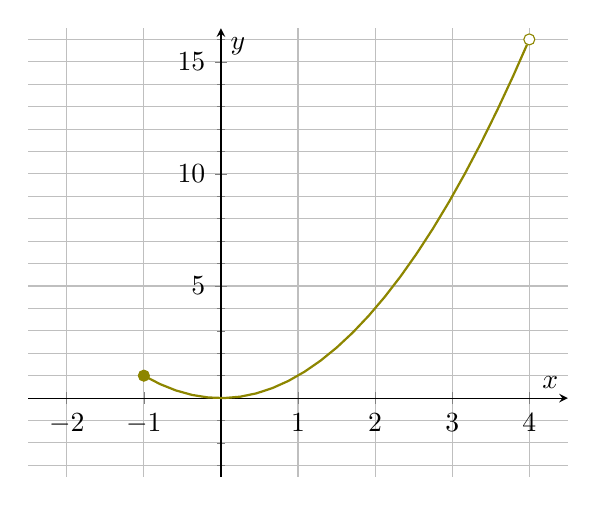
\begin{tikzpicture}
	\begin{axis}
	[axis lines = center, 
	xmin = -2.5, xmax = 4.5,
	ymin = -3.5, ymax = 16.5,
	xtick = {-3,-2,...,4,5},
	ytick = {-5,0,...,15,20},
	minor y tick num = 4,
	grid = both,
	xlabel = $x$, ylabel = $y$,
	]
		\addplot[color = olive, thick, domain = -1:4] {x^2};	
		\filldraw[color = white](axis cs: 4,16) circle (2pt);
		\filldraw[color = olive](axis cs: -1,1) circle (2pt);
		\draw[color = olive](axis cs: 4,16) circle (2pt);	
	\end{axis}
\end{tikzpicture}
}		
\resizebox{0.45\textwidth}{!}{
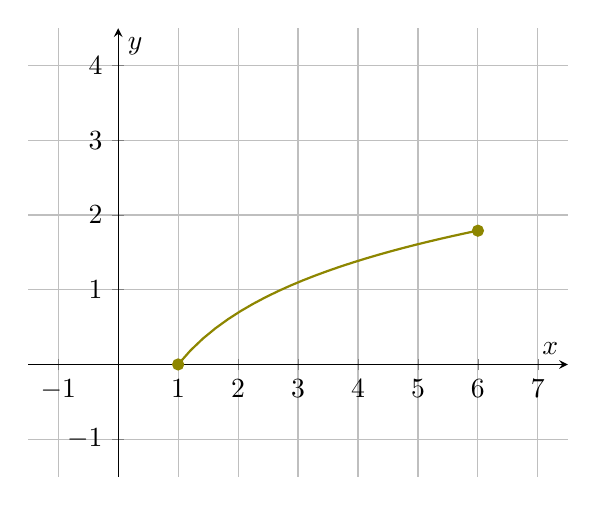
\begin{tikzpicture}
	\begin{axis}
	[axis lines = center, 
	xmin = -1.5, xmax = 7.5,
	ymin = -1.5, ymax = 4.5,
	grid = both,
	xtick = {-3,-2,...,6,7},
	ytick = {-3,-2,...,6,7},
	xlabel = $x$, ylabel = $y$
	]
		\addplot[color = olive, thick, domain = 1:6] {ln(x)};	
		\filldraw[color = olive](axis cs: 1,0) circle (2pt);
		\filldraw[color = olive](axis cs: 6, 1.79 ) circle (2pt);
	\end{axis}
\end{tikzpicture}
}
\resizebox{0.45\textwidth}{!}{
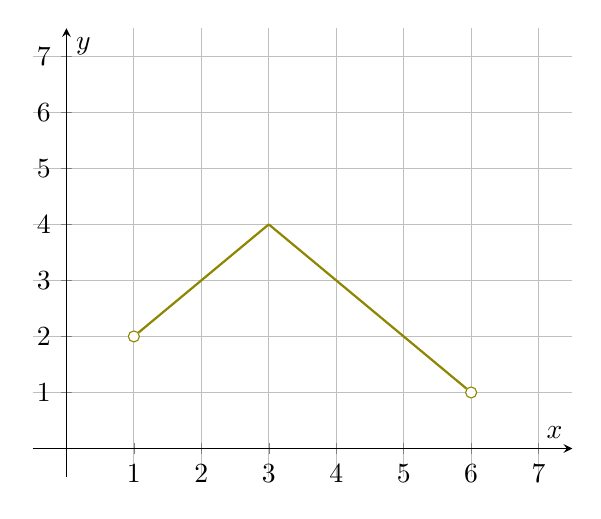
\begin{tikzpicture}
	\begin{axis}
	[axis lines = center, 
	xmin = -0.5, xmax = 7.5,
	ymin = -0.5, ymax = 7.5,
	grid = both,
	xtick = {-3,-2,...,6,7},
	ytick = {-3,-2,...,6,7},
	xlabel = $x$, ylabel = $y$
	]
		\addplot[color = olive, thick, domain = 1:3] {x + 1};
		\addplot[color = olive, thick, domain = 3:6] {-x + 7};	
		\filldraw[color = white](axis cs: 1,2) circle (2pt);
		\filldraw[color = white](axis cs: 6,1) circle (2pt);
		\draw[color = olive](axis cs: 1,2) circle (2pt);
		\draw[color = olive](axis cs: 6,1) circle (2pt);
	\end{axis}
\end{tikzpicture}
}
\resizebox{0.45\textwidth}{!}{
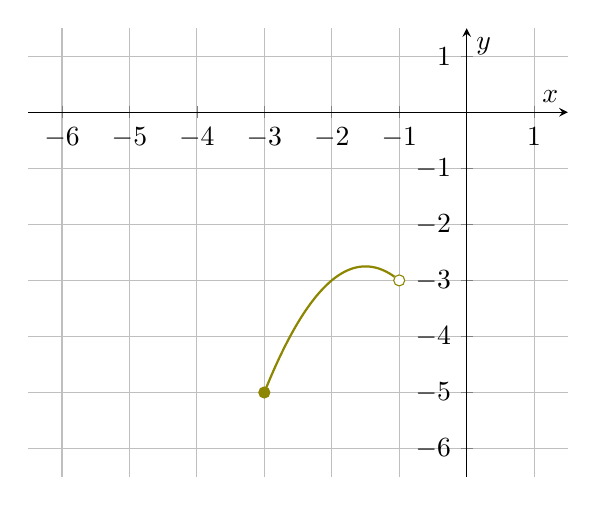
\begin{tikzpicture}
	\begin{axis}
	[axis lines = center, 
	xmin = -6.5, xmax = 1.5,
	ymin = -6.5, ymax = 1.5,
	grid = both,
	xtick = {-6,-5,...,6,7},
	ytick = {-6,-5,...,6,7},
	xlabel = $x$, ylabel = $y$
	]
		\addplot[color = olive, thick, domain = -3:-1, samples = 200] {-x^2-3*x-5};	
		\filldraw[color = white](axis cs: -1,-3) circle (2pt);
		\filldraw[color = olive](axis cs: -3,-5) circle (2pt);
		\draw[color = olive](axis cs: -1,-3) circle (2pt);
	\end{axis}
\end{tikzpicture}
}
\resizebox{0.45\textwidth}{!}{
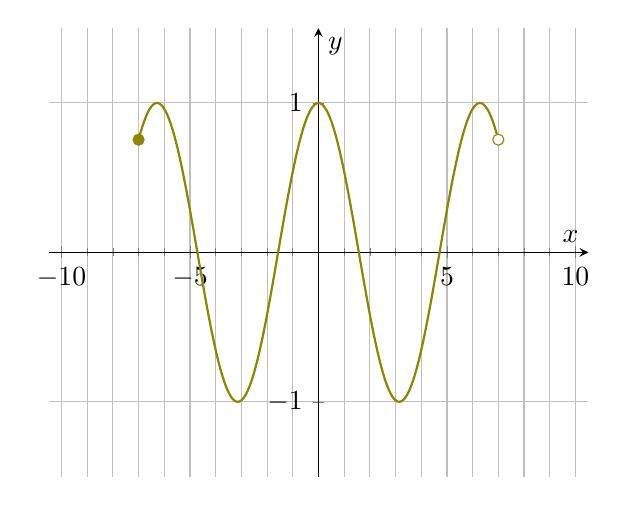
\begin{tikzpicture}
	\begin{axis}
	[axis lines = center, 
	xmin = -10.5, xmax = 10.5,
	ymin = -1.5, ymax = 1.5,
	grid = both,
	xtick = {-15,-10,...,10,15},
	minor x tick num = 4,
	ytick = {-1,0,1},
	xlabel = $x$, ylabel = $y$
	]
		\addplot[color = olive, thick, domain = -7:7, samples = 200] {cos(deg(x))};	
		\filldraw[color = white](axis cs: 7,0.754) circle (2pt);
		\filldraw[color = olive](axis cs: -7,0.754) circle (2pt);
		\draw[color = olive](axis cs: 7,0.754) circle (2pt);
	\end{axis}
\end{tikzpicture}
}
\end{center}

\subsection*{Opgave 2}
Tegn følgende funktioner i Maple og bestem deres ekstrema. Afgør desuden, om de er lokale eller globale ekstrema.
\begin{align*}
	&1) \  f(x) = x^2 &   &2) \  f(x) = x^3 + 7 x^2 - 36 \\
	&3) \  f(x) = \sqrt{x^2-5x+10} &   &4) \  f(x) = x\cdot \cos(x), \ -10 \leq x \leq 10 \\
	&5) \  f(x) = \sin(x), \ 0 < x < 20 &   &6) \  f(x) = \begin{cases} x^2, \ &\textnormal{hvis }x \geq 7, \\
	-2x + 7, \ &\textnormal{hvis }x < 7.
	\end{cases}
\end{align*}

\subsection*{Opgave 3}

Bestem først ekstrema for følgende funktioner og opskriv derefter deres monotoniforhold.


\begin{center}
\resizebox{0.45\textwidth}{!}{
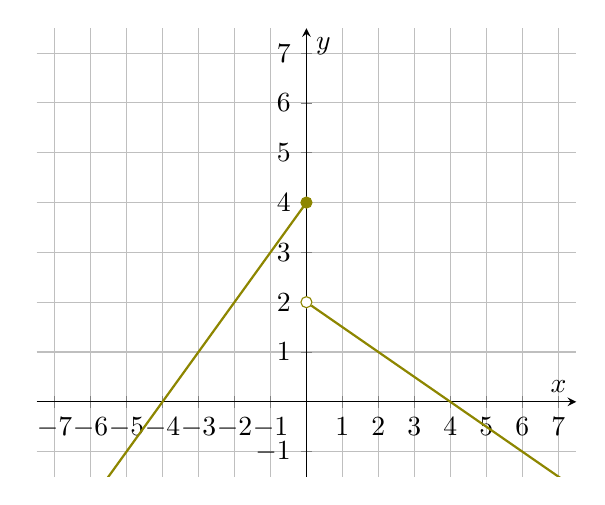
\begin{tikzpicture}
	\begin{axis}
	[axis lines = center, 
	xmin = -7.5, xmax = 7.5,
	ymin = -1.5, ymax = 7.5,
	grid = both,
	xtick = {-7,-6,...,6,7},
	ytick = {-3,-2,...,6,7},
	xlabel = $x$, ylabel = $y$
	]
		\addplot[color = olive, thick, domain = -8:0] {x + 4};
		\addplot[color = olive, thick, domain = 0:8] {-0.5*x + 2};	
		\filldraw[color = olive](axis cs: 0,4) circle (2pt);
		\filldraw[color = white](axis cs: 0, 2 ) circle (2pt);
		\draw[color = olive](axis cs: 0, 2 ) circle (2pt);
	\end{axis}
\end{tikzpicture}
}
\resizebox{0.45\textwidth}{!}{
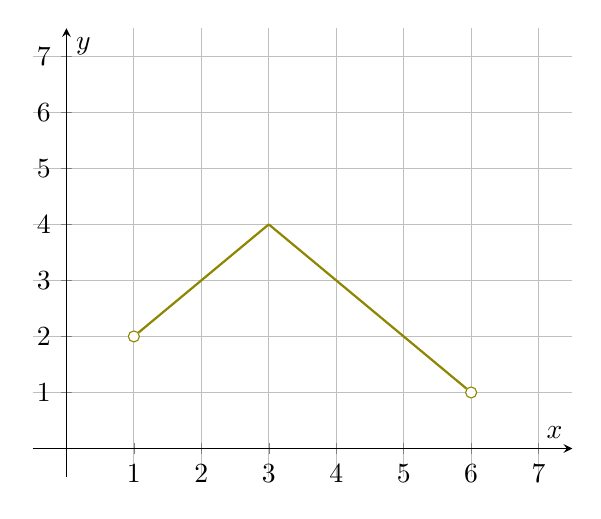
\begin{tikzpicture}
	\begin{axis}
	[axis lines = center, 
	xmin = -0.5, xmax = 7.5,
	ymin = -0.5, ymax = 7.5,
	grid = both,
	xtick = {-3,-2,...,6,7},
	ytick = {-3,-2,...,6,7},
	xlabel = $x$, ylabel = $y$
	]
		\addplot[color = olive, thick, domain = 1:3] {x + 1};
		\addplot[color = olive, thick, domain = 3:6] {-x + 7};	
		\filldraw[color = white](axis cs: 1,2) circle (2pt);
		\filldraw[color = white](axis cs: 6,1) circle (2pt);
		\draw[color = olive](axis cs: 1,2) circle (2pt);
		\draw[color = olive](axis cs: 6,1) circle (2pt);
	\end{axis}
\end{tikzpicture}
}
\resizebox{0.45\textwidth}{!}{
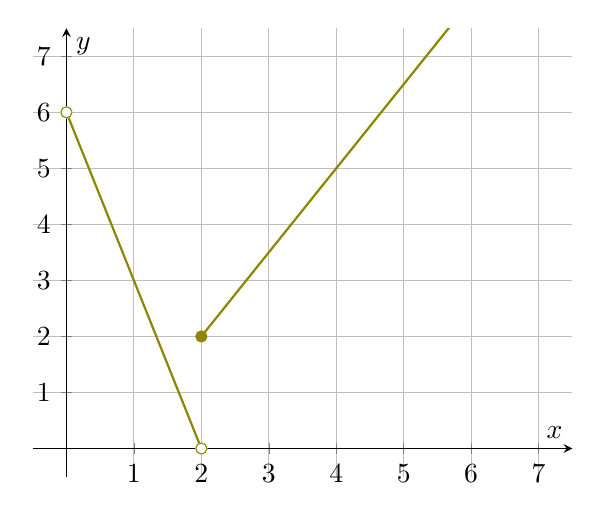
\begin{tikzpicture}
	\begin{axis}
	[axis lines = center, 
	xmin = -0.5, xmax = 7.5,
	ymin = -0.5, ymax = 7.5,
	grid = both,
	xtick = {-3,-2,...,6,7},
	ytick = {-3,-2,...,6,7},
	xlabel = $x$, ylabel = $y$
	]
		\addplot[color = olive, thick, domain = 0:2] {-3*x + 6};
		\addplot[color = olive, thick, domain = 2:6] {1.5*x - 1};	
		\filldraw[color = white](axis cs: 0,6) circle (2pt);
		\filldraw[color = white](axis cs: 2,0) circle (2pt);
		\draw[color = olive](axis cs: 0,6) circle (2pt);
		\draw[color = olive](axis cs: 2,0) circle (2pt);
		\filldraw[color = olive] (axis cs: 2,2) circle (2pt);
	\end{axis}
\end{tikzpicture}
}
\resizebox{0.45\textwidth}{!}{
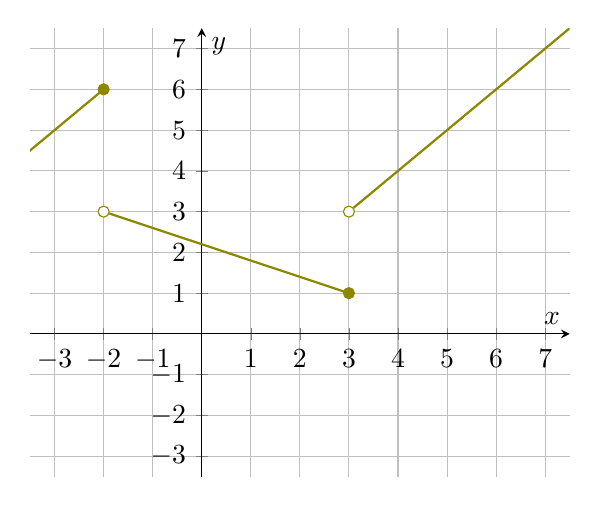
\begin{tikzpicture}
	\begin{axis}
	[axis lines = center, 
	xmin = -3.5, xmax = 7.5,
	ymin = -3.5, ymax = 7.5,
	grid = both,
	xtick = {-3,-2,...,6,7},
	ytick = {-3,-2,...,6,7},
	xlabel = $x$, ylabel = $y$
	]
		\addplot[color = olive, thick, domain = -2:3] {-2/5*x+2.2};
		\addplot[color = olive, thick, domain = 3:10] {x};	
		\addplot[color = olive, thick, domain = -4:-2] {x + 8};	
		\filldraw[color = white](axis cs: -2,3) circle (2pt);
		\filldraw[color = olive](axis cs: 3,1) circle (2pt);
		\draw[color = olive](axis cs: -2,3) circle (2pt);
		\filldraw[color = white](axis cs: 3,3) circle (2pt);
		\draw[color = olive](axis cs: 3,3) circle (2pt);
		\filldraw[color = olive](axis cs: -2,6) circle (2pt);
	\end{axis}
\end{tikzpicture}
}
\end{center}

\subsection*{Opgave 4}
Tegn følgende funktioner i Maple og bestem monotoniforholdene for dem

\begin{align*}
	&1) \  f(x) = -x^2+5x-9 &   &2) \  f(x) = -x^4 + 7 x^3 - 36x^2+14x-10 \\
	&3) \  f(x) = \ln(x^5-9x^4)&   &4) \  f(x) = -x\cdot \sin(x), \ -10 \leq x \leq 10 \\
	&5) \  f(x) = \sin(x), \ -10 < x < 4 &   &6) \  f(x) = \begin{cases} \sqrt{-x}, \ &\textnormal{hvis }x \leq -5, \\
	x^2, \ &\textnormal{hvis }x > 5.
	\end{cases}
\end{align*}

\subsection*{Opgave 5}
Hvis en funktion er strengt monoton på et interval, kan du så gennemskue, om funktionen er surjektiv, injektiv eller bijektiv?
